\section*{Exercise (vii)}

Based on the $N = 1000$ simulated paths from Exercise~(vi), we estimate the expected life annuity benefit $\mathbb{E}[Y(t) \mid X(m)]$ at each time point by the sample mean across paths:
\[
  \hat{\mathbb{E}}[Y(t) \mid X(m)] = \frac{1}{N}\sum_{n=1}^{N} Y^{(n)}(t).
\]

\begin{figure}[H]
    \centering
    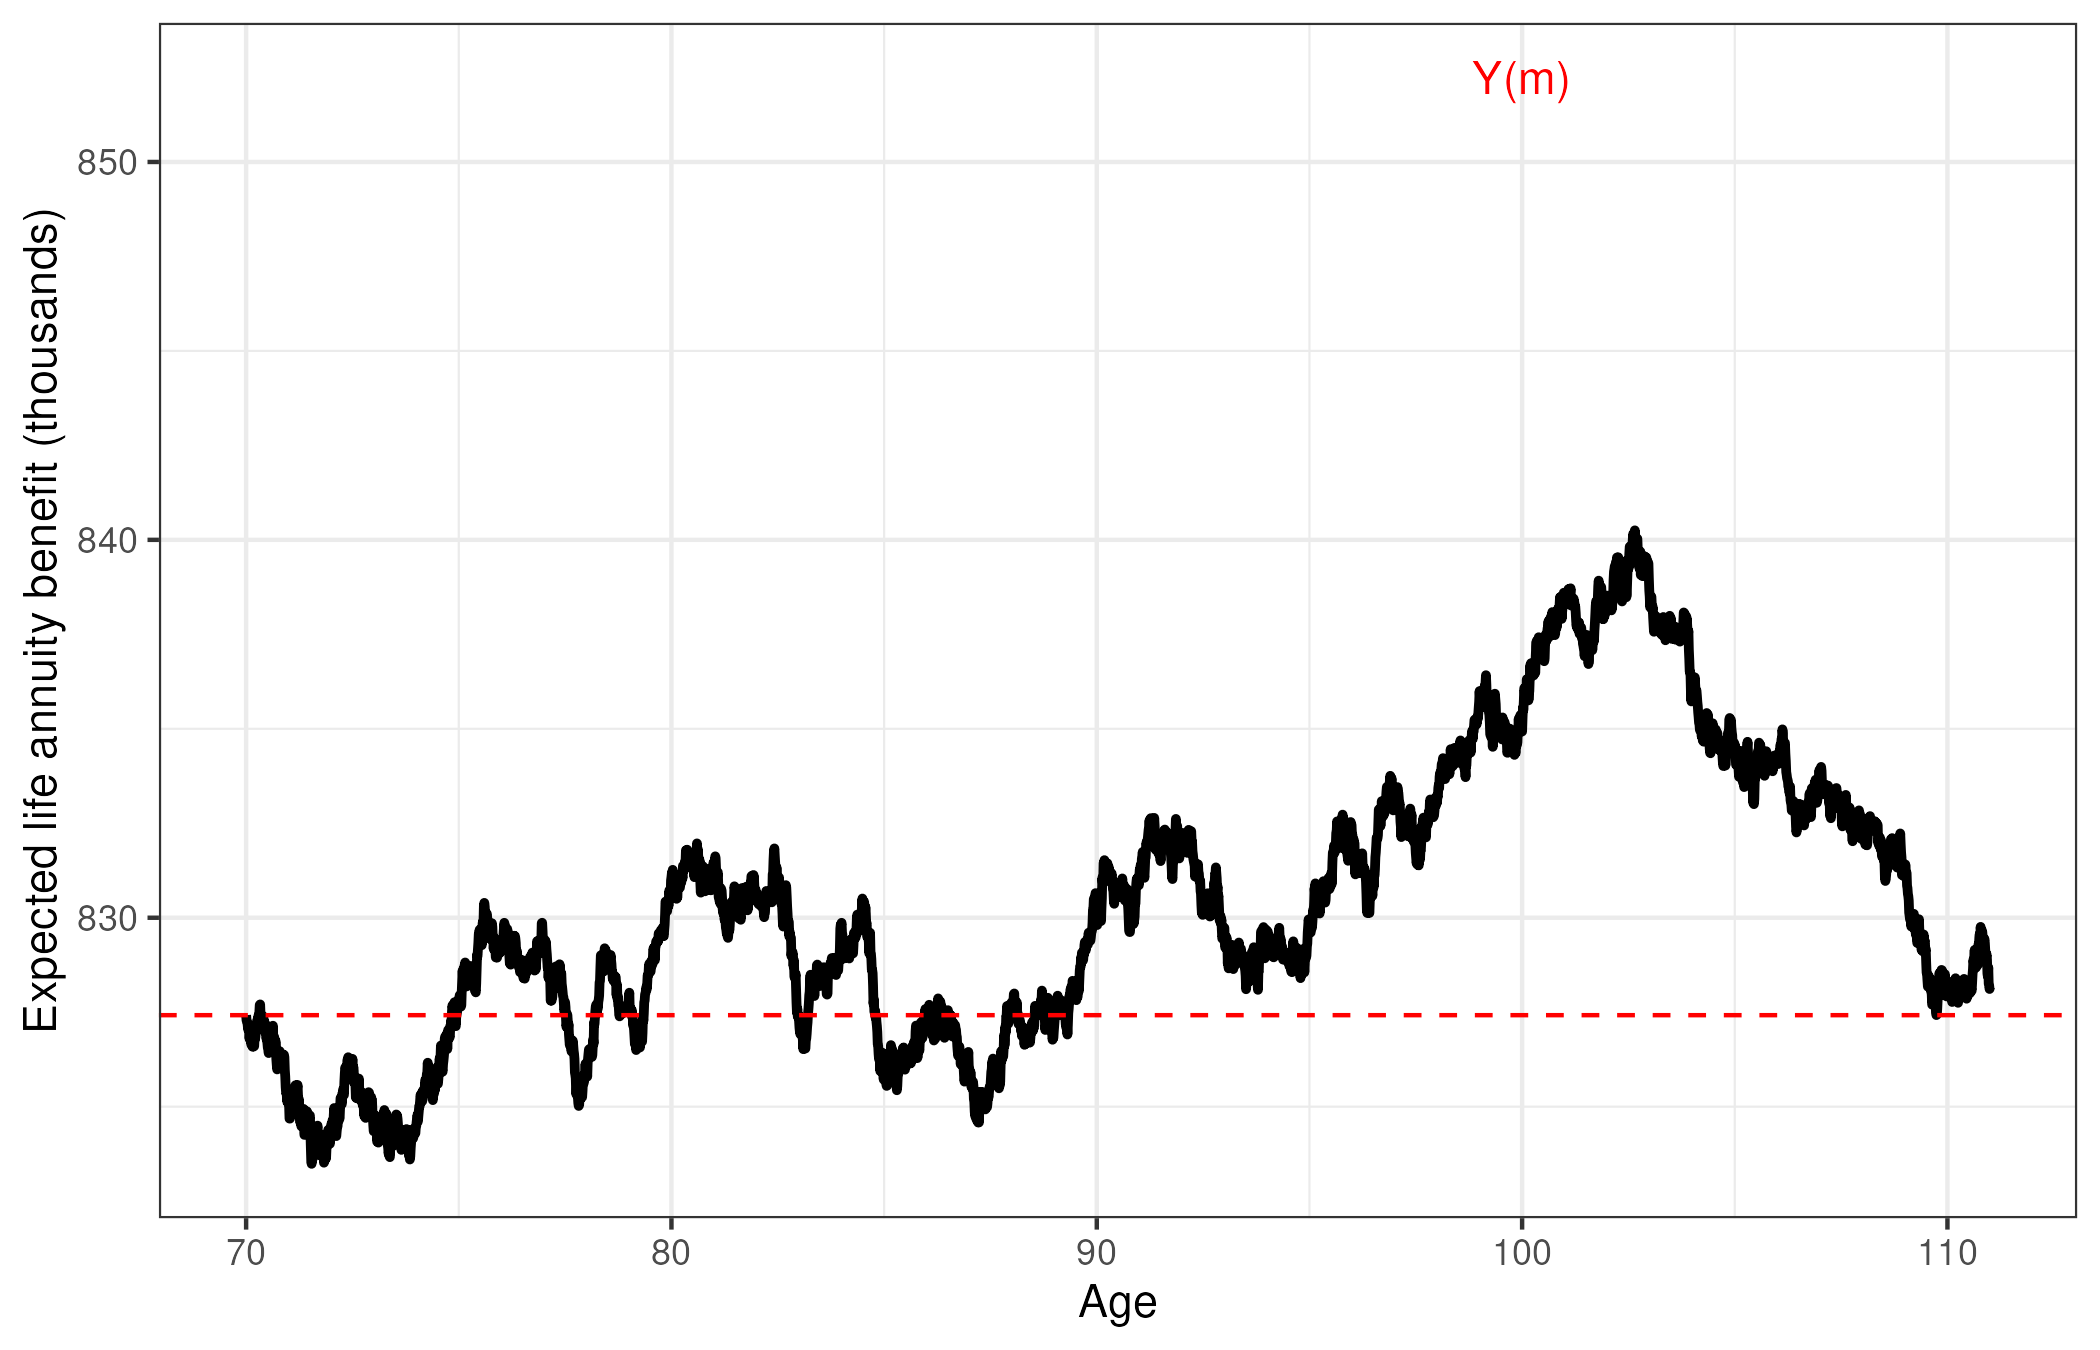
\includegraphics[width=0.75\linewidth]{Pictures/ExpectedAnnuity.png}
    \caption{Estimated expected life annuity benefit $\mathbb{E}[Y(t) \mid X(m)]$ over time. The dashed red line marks $Y(m)$.}
\end{figure}

We observe that the expected payout profile is approximately \emph{flat} over the entire retirement period. This is consistent with the theoretical result from Exercise~(v): since $\tilde{r}(t) = \pi(t)\alpha + (1-\pi(t))r$ and $\tilde{\mu}(t) = \mu(t)$, the drift of $Y$ is zero and $Y$ is an exponential martingale, so $\mathbb{E}[Y(t) \mid X(m)] = Y(m)$ for all $t \geq m$. The small fluctuations visible in the plot are Monte Carlo noise from the finite sample of $N = 1000$ paths.

In practice, this flat expected profile means that, on average, the insured receives the same benefit throughout retirement. However, as seen in Exercise~(vi), individual paths exhibit substantial variability around this expectation---the insured bears significant investment risk. A more conservative calculation basis (with $\tilde{r}(t) < \pi(t)\alpha + (1-\pi(t))r$) would instead produce an increasing expected payout profile, starting lower but growing over time, which could be preferable from a product design perspective.

